\chapter{Descrizione dell'architettura ROS}
\label{cha:descrizionearchros}
Nel capitolo precedente ho approfondito il linguaggio Prolog e come ho sviluppato il caso di studio. In questo capitolo verrà descritta l'architettura ROS utilizzata per la simulazione e la possibile applicazione reale.
In particolare verrà data una breve descrizione di cosa è ROS e come funziona, per poi passare alla descrizione dell'architettura utilizzata per la simulazione concludendo poi con una sezione dedicata alle difficoltà incontrate. Iniziamo quindi con una breve introduzione a ROS.

\section{Introduzione a ROS}
\label{sec:introduzione_ros}
ROS (Robot Operating Systems) è un framework opensource per lo sviluppo e la programmazione di robot. ROS implementa drivers e algoritmi che sono lo stato dell'arte in robotica grazie anche alla community che negli anni si è formata e ingrandita.
Essendo infatti un progetto opensource, ROS è sviluppato e mantenuto in parte dalla community stessa. Questo è un grosso vantaggio; infatti così facendo il supporto verso nuovi hardware sarà sempre al passo con i tempi. Inoltre la community è molto attiva per consigli e aiuti sia per i meno esperti che non, e questo sicuramente è un punto a suo favore.
Per realizzare questo capitolo mi sono documentato dalla wiki del progetto \cite{rossite} e dall'articolo \textit{ROS: an open-source Robot Operating System} \cite{quingley2009ros}.

Iniziamo quindi introducendo i concetti principali di un architettura ROS.

\subsection{Nodi}
\label{subsec:nodi}
Con il termine nodo si intende un processo che esegue un compito specifico, questo utilizza ROS per comunicare con gli altri nodi. I nodi possono pubblicare oppure iscriversi ad un topic, inoltre possono offrire un servizio o richiederlo. 

In ROS1, quello che è stato utilizzato per la simulazione, è necessario che ci sia un nodo master. Per avviarlo è necessario digitare il comando \verb+roscore+. Questo avrà il compito di coordinare le attività del nostro sistema distribuito. Più in dettaglio dovrà: tenere traccia dei nomi dei nodi ecc. tramite il registro dei nomi, fornire un servizio di ricerca consultabile dai nodi stessi, tenere traccia dei topic e dei messaggi che vengono pubblicati e infine fornire il servizio del parameter server.
I messaggi e le chiamate di servizio non passano dal nodo master, infatti la comunicazione in ROS è peer-to-peer. Questo permette di avere un sistema distribuito e scalabile. Inoltre, essendo peer-to-peer, non è necessario che tutti i nodi siano attivi contemporaneamente, infatti è possibile che un nodo si sottoscriva ad un topic anche se il nodo che lo pubblica non è ancora attivo. Questo permette di avere un sistema molto flessibile e scalabile.

In conclusione un nodo è un processo che esegue un compito specifico e che comunica con gli altri nodi attraverso i topic, i servizi e il parameter server.
\subsection{Topics}
\label{subsec:topics}
In ROS i topic sono un canale di comunicazione asincrona che permette ai nodi di scambiarsi messaggi. I Topic in ROS seguono l'architettura \textit{publisher-subscriber}, un nodo quindi può pubblicare messaggi su un topic specifico mentre uno o più nodi si sottoscrivono al topic per ricevere i messaggi.
I topic in ROS sono organizzati gerarchicamente e sono identificati da un nome univoco. La gerarchia permette di organizzarli in base diversi aspetti dell'applicazione o dei dati che vengono scambiati. 
Come detto prima la comunicazione è asincrona, quindi il nodo pubblicante non aspetta una risposta immediata dal nodo abbonato.
Con il comando \verb+rostopic list+ possiamo avere una panoramica dei topic che sono attivi nella nostra rete. Con il comando \verb+rostopic echo <nometopic>+, invece, possiamo vedere i messaggi che vengono pubblicati su un topic specifico. In questo modo possiamo capire se i topic sono attivi e quindi se i nodi stanno comunicando tra di loro.

In conclusione i topic sono quindi un canale di comunicazione asincrona che permette ai nodi di scambiarsi messaggi. Questi sono organizzati gerarchicamente e sono identificati da un nome univoco.
\subsection{Messaggi}
\label{subsec:messaggi}
I messaggi sono i dati che vengono scambiati dai nodi attraverso i topic. Questi possono essere di vari tipi e sono definiti in un file \verb+.msg+. Questo file contiene la definizione del messaggio, ovvero il nome del messaggio e i campi che lo compongono. I campi possono essere di vari tipi, come ad esempio: interi, stringhe, array, ecc.
La personalizzazione dei messaggi permette all'utente un controllo totale della propria applicazione riuscendo a definire i messaggi che meglio si adattano alle proprie esigenze.
Con il comando \verb+rostopic info <nometopic>+ possiamo avere una panoramica dei messaggi che vengono scambiati su un topic specifico. Inoltre con il comando \verb+rosmsg show <nomemsg>+ possiamo avere i dettagli di come è composto il messaggio specifico.

In conclusione i messaggi sono i dati che vengono scambiati dai nodi attraverso i topic. Questi sono definiti in un file \verb+.msg+ e possono essere di vari tipi per adattarsi alle esigenze dell'utente.
\subsection{ROS services e parameter server}
\label{subsec:servandparam}
L'ultima nozione fondamentale da sapere sull'architettura ROS è il concetto di \textit{ROS service} e \textit{parameter server}. I ROS service sono un modo alternativo per comunicare in ROS; questi a differenza dei topic sono sincroni. Questo significa che il nodo che richiede un servizio deve aspettare che il nodo che lo fornisce risponda. 
Anche i ROS services sono identificati da un nome univoco e vengono chiamati/richiesti appunto da esso. Una volta che un nodo richiede un servizio questo bloccherà la sua esecuzione, riprendendola solamente quando il servizio sarà stato fornito.
I servizi in ROS vengono usati principalmente se è necessario ottenere una risposta immediata, ad esempio la richiesta di dati di configurazione, l'esecuzione di operazioni complesse oppure la richiesta di operazioni specifiche.

Il \textit{parameter server} in ROS è un componente centrale che consente ai nodi di memorizzare e recuperare dei parametri di sistema. Può essere inteso come un database centralizzato in cui i nodi possono leggere e scrivere i valori dei parametri.
Questi parametri possono essere usati per configurare il comportamento dei nodi, impostare valori costanti o condividere dati tra i componenti del sistema. I parametri sono organizzati tramite dei namespace così da semplificare la ricerca e la gerarchia.

\subsection{Esempio rete ROS}
\label{subsec:esempio_rete_ros}
Per capire meglio come sono strutturati questi componenti utilizziamo il famoso simulatore \textit{turtlesim} e generiamo il grafo della rete tramite il comando \verb+rosrun rqt_graph rqt_graph+. Il grafo generato è il seguente (figura \ref{fig:turtlesim}).
\begin{figure}[h!]
    \centering
    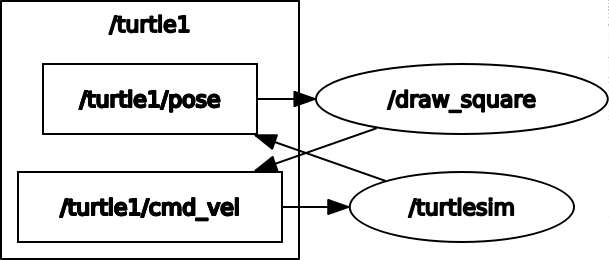
\includegraphics[scale=0.5]{images/turtlesim.png}
    \caption{Grafo della rete turtlesim}
    \label{fig:turtlesim}
\end{figure}
I nodi sono identificati dagli ovali mentre i topic sono identificati dai rettangoli. Vediamo come i due nodi turtlesim e draw\_square comunicano tra loro tramite i topic \verb+/turtle1/pose+ e \verb+/turtle1/cmd_vel+. Il nodo /draw\_square pubblica sul topic /cmd\_vel la traiettoria per la "tartaruga", questa sarà poi inviata al nodo del simulatore per poi essere eseguita. Quest'ultimo a sua volta pubblicherà la posa del robot al topic /pose che sarà poi letto dal nodo /draw\_square per recuperare la posizione del robot e disegnare la traiettoria.
Il risultato è visibile in figura \ref{fig:turtlesimes}.
\begin{figure}[h!]
    \centering
    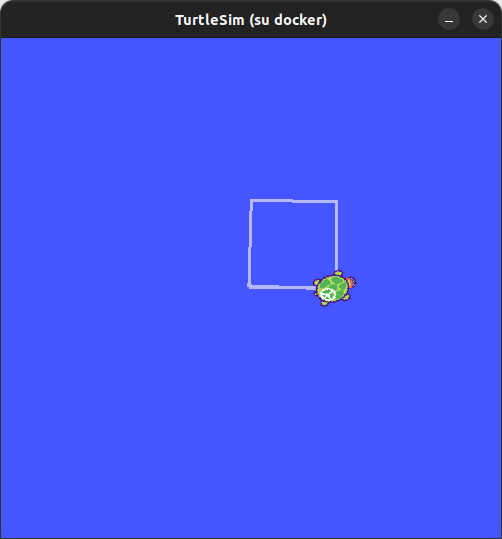
\includegraphics[scale=0.4]{images/turtlesimes.png}
    \caption{Esempio di simulazione turtlesim}
    \label{fig:turtlesimes}
\end{figure}

Passiamo ora a vedere come è strutturata la rete per il mio caso di studio
\section{Architettura utilizzata}
\label{sec:architettura_utilizzata}
In questa sezione mi concentrerò nell'illustrazione dell'architettura utilizzata per il mio caso di studio andando a definire le milestone indicate nel capitolo \ref{cha:descrizionecasostudio}.
Analizziamo quindi la terza e la quarta milestone.

\subsection{Terza milestone: Wrapping codice Prolog}
\label{subsec:wrappping}
In informatica, il termine wrapping si riferisce a una tecnica o un processo in cui un elemento o un oggetto viene incapsulato da un altro strato o struttura.
Questo viene fatto per rendere l'interfaccia del programma più semplice oppure per astrarre maggiormente la stessa. 

Nel mio caso il codice Prolog è stato incapsulato grazie alla libreria PySwip \cite{pyswip}; questa fornisce un interfaccia per comunicare con il motore di inferenza SWI-Prolog tramite il linguaggio Python.
In questo modo ho potuto utilizzare il codice Prolog come se fosse una libreria Python, rendendo l'interfaccia più semplice e più comprensibile. 
Oltre al fattore di semplicità, questo è stato fatto per poi creare il nodo ROS utilizzando la client library rospy.
Il processo di wrapping è molto semplice, si utilizzano le API messe a disposizione da PySwip per interrogare la base di conoscenza, si ottengono i risultati e si utilizzano per creare il nodo ROS.
Qui di seguito riporto come è stato fatto il wrapping del codice per il mio progetto, il file \verb+prolog_node.py+ contiene il seguente codice:
\begin{lstlisting}[language=Python]
from pyswip import Prolog
prolog = Prolog()
prolog.consult("block_world.pl")
result = list(prolog.query("get_blocks(Blocks)"))
result = list(prolog.query(
                "once(pillar(" + x + "," + y + "," + z + 
                "," + h + "," + w + "," + d + ", Actions))"))
\end{lstlisting}
Il codice riportato non corrisponde riga per riga a quello completo, ho riportato soltanto dove viene utilizzato il bridge. Nella prima istruzione dalla libreria PySwip viene importata la classe Prolog, questa ci permette di interrogare la base di conoscenza. Viene istanziato quindi un oggetto della medesima classe e viene caricato il file Prolog tramite il metodo \verb+consult+.
Nelle due righe successive vengono svolte due query: una serve a recuperare la lista dei blocchi presenti nella scena, l'altra invece serve a recuperare la lista di azioni da eseguire per risolvere il problema. Il metodo \verb+query+ restituisce un generatore, per questo motivo viene utilizzato il metodo \verb+list+ per convertirlo in una lista. 

Come detto prima, il processo di wrapping non è complesso e come si può ben vedere, è intuitivo e compatto. 
Per la realizzazione di questa milestone ho impiegato poco meno di una settimana, in questo caso i primi giorni sono serviti per ricercare una libreria che mi permettesse di fare il wrapping del codice Prolog, mentre i restanti giorni sono serviti per capire come utilizzare la libreria e per scrivere il codice.
Siccome al momento di realizzazione di questa milestone, circa il 18 giugno, l'architettura ROS non era stata ancora creata, ho dovuto creare un nodo di prova per testare il wrapping del codice Prolog. 
Questo è consultabile nella mia repository ed è il file \verb+python_node_poc.py+. Questo file conteneva una \textit{proof of concept} di ciò che volevo realizzare, ovvero un nodo che interrogasse la base di conoscenza e che mostrasse i risultati ottenuti. 
Ho quindi realizzato il programma, questo chiedeva all'utente i dati in input per il predicato \verb+pillar/7+ e poi interrogava la base di conoscenza. I risultati poi venivano mostrati tramite un interfaccia grafica minimale realizzata con la libreria Tkinter.

Sviluppata questa milestone, mancava soltanto la creazione della rete ROS e la simulazione. 


\subsection{Quarta milestone: Simulazione}
\label{subsec:simulation}
Questa è l'ultima milestone, la realizzazione della simulazione in ROS e Gazebo. Questa, pur essendo secondaria al mio progetto di tesi, è stata molto importante perchè offre un esempio pratico del caso di studio.
Per la realizzazione della simulazione ho utilizzato ROS Noetic e Gazebo, quest'ultimo è un simulatore fisico 3D open source che permette di simulare robot, oggetti e ambienti.
La simulazione del UR5 è stata realizzata utilizzando il framework \textit{locosim} \cite{focchi2023locosim}, questo rende disponibile out-of-the-box il modello del robot con annessi controller per la simulazione in Gazebo.
Per questa milestone quindi ho dovuto sviluppare i due nodi ROS che si occupano di interrogare la base di conoscenza e di eseguire le azioni ottenute.

L'architettura ROS ideata per il mio caso di studio è illustrata in figura \ref{fig:archros}. Come si vede dalla figura i nodi sono 3: il task planner, il motion planner e il nodo per la simulazione del UR5. 
\begin{figure}[t]
    \centering
    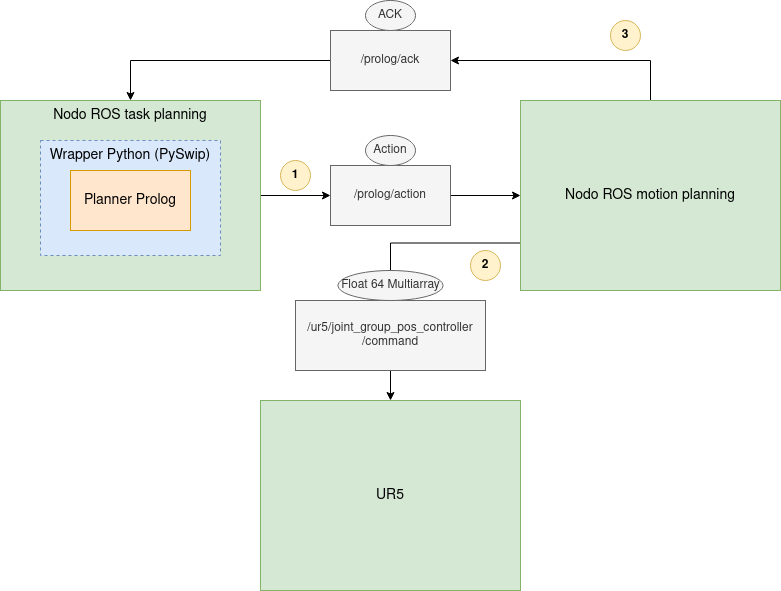
\includegraphics[scale=0.5]{images/ArchROS.drawio.png}
    \caption{Architettura ROS. In verde ci sono i nodi mentre in grigio chiaro i topic con i relativi messaggi.}
    \label{fig:archros}
\end{figure}
In particolare, quelli sviluppati da me sono appunto il nodo in Prolog e quello di motion planning. Iniziamo descrivendo appunto quest'ultimo.

\subsubsection{Motion planner}
\label{subsubsec:motionplanner}
Il nodo di motion planning ha come obiettivo quello di pianificare ed eseguire i movimenti che il robot deve compiere per effettuare le azioni ottenute dal task planner.
Ci sono varie strategie per realizzarlo, io ho scelto di utilizzare una strategia relativamente semplice da eseguire ma allo stesso tempo completa per tutti i movimenti che il robot deve compiere. Essa è composta principalmente dagli algoritmi di cinematica e  dalla interpolazione cubica di punti nello spazio.
Partiamo descrivendo i primi due concetti, cinematica diretta e inversa, per poi passare alla generazione della traiettoria.
La \textit{cinematica diretta} consente di trovare la posizione e l'orientamento attuale dell'end effector\footnote{End effector: parte finale di un manipolatore robotico, nel mio caso un gripper a due dita.} di un robot in funzione delle posizioni dei suoi giunti. 
Questa solitamente viene utilizzata per localizzare l'end effector nello spazio, io, però, non l'ho mai utilizzata siccome conoscevo a priori la sua configurazione di partenza dato che è definita dall'utente. Ho introdotto questo concetto solamente per completezza e per capire meglio la cinematica inversa.
Questa, come suggerisce il nome, svolge il compito opposto, ovvero trovare le posizioni dei giunti in funzione della posizione e dell'orientamento del end effector del robot.
Di questa ne ho fatto ampio uso nel mio nodo siccome mi permetteva di trovare la configurazione dei giunti in funzione della posizione del blocco da afferrare.
Questo problema non ha una unica soluzione ma, nel nostro caso, ne ha 8. Quindi ho adottato la strategia di scelta della soluzione in base alla distanza rispetto alla configurazione precedente. Questo mi ha permesso di avere una continuità nei movimenti del robot.
La distanza veniva calcolata attraverso la norma delle due configurazioni e la soluzione scelta era quella che minimizzava la distanza.

Minimizzata la distanza e trovata la configurazione dei giunti, il robot doveva eseguire il movimento. Per fare ciò ho utilizzato una interpolazione cubica di punti nello spazio. Questa serve a trovare tutte le configurazioni necessarie per arrivare da un punto \textit{A} ad un punto \textit{B} in un certo intervallo di tempo e compiendo un movimento fluido. 
Per la sua realizzazione mi sono servito del paper di Shuang Fang et al. \cite{8941347}, in particolare la parte in cui descriveva la creazione di, appunto, una traiettoria cubica.

Avendo la cinematica e la traiettoria funzionante ho dovuto solamente pensare ad un modo di gestire le azioni ottenute dal task planner. L'azione \textit{move} l'ho voluta gestire con un semplice movimento con dei punti di controllo intermedi. In particolare ho voluto strutturare l'azione nel seguente modo:
\begin{enumerate}
    \item Il braccio robotico approccia il blocco da afferrare stando ad una altezza prefissata.
    \item Il braccio robotico si abbassa fino a toccare il blocco e lo afferra.
    \item Il braccio torna a posizione 1.
    \item Il braccio approccia la posizione finale ad una altezza prefissata.
    \item Il braccio si abbassa fino a toccare il piano e rilascia il blocco.
    \item Il braccio torna a posizione 4.
\end{enumerate}
Questa è la strategia che ho voluto adottare per l'istruzione \textit{move}.

Per l'istruzione \textit{rotate}, invece, il movimento dipende dall'orientamento di partenza del blocco. 
Ogni orientamento avrà la sua strategia per ruotare in posizione corretta, cioè con la base verso il tavolo, il blocco.

Calcolate le posizioni dei giunti e la traiettoria, il nodo di motion planning invia i comandi al robot per eseguire il movimento.
Eseguito quest'ultimo, il nodo di motion planning invia un messaggio al task planner per notificare l'esecuzione dell'azione e per permettere al task planner di proseguire con la prossima istruzione (punto 3 in figura \ref{fig:archros}).

La parte di motion planning dipende dalle istruzioni generate dal task planner. Vediamo quindi come queste sono estrapolate dal programma Prolog e come sono inviate al nodo di motion planning
\subsubsection{Task planner}
\label{subsubsec:taskplanner}
Il nodo di task planning ha come obiettivo quello di interrogare la base di conoscenza e di estrapolare le azioni da eseguire per portare a termine il programma Prolog.
Come visto prima, questo nodo è scritto in python e utilizza la libreria \textit{pySwip} per interrogare la base di conoscenza. 
Ricevuto il risultato questo viene processato tramite la libreria di espressioni regolari \textit{re} per estrapolare le azioni da eseguire. 
Estrapolate le azioni, queste vengono inviate con il messaggio appositamente creato al nodo di motion planning. Il messaggio in questione si chiama \textit{action} e contiene il nome dell'azione da eseguire e i parametri necessari per eseguirla cioè le posizioni iniziali e finali e l'orienatamento iniziale.
Inviato il messaggio, il nodo di task planning si mette in attesa di una risposta dal nodo di motion planning per poter proseguire con la prossima azione.

\section{Difficoltà incontrate}
\label{sec:difficoltaros}
Durante lo sviluppo della simulazione ho incontrato diverse difficoltà; molte, se non la totalità di queste, legate al simulatore Gazebo. In questa sezione descriverò le principali difficoltà incontrate e come le ho risolte.

Durante lo sviluppo mi sono scontrato con due grandi imprevisti, tutti e due legati al motore di simulazione Gazebo.
Il primo era legato alla simulazione del \textit{grasping}, ovvero l'azione di afferrare un oggetto con il robot. Questo è un problema ben noto alla comunità di ricerca e sono stati sviluppati diversi metodi per risolverlo.
Uno tra questi è l'utilizzo di un plugin chiamato \textit{gazebo\_grasp\_plugin} che permette di simulare il grasping di un oggetto con il robot. Questo crea un \textit{link} dinamico tra il robot e l'oggetto che permette di simulare il movimento di afferramento. Questo verrà creato quando il robot applicherà una certa forza al blocco e verrà eliminato quando questa forza verrà rimossa.
Un accorgimento che ho dovuto prendere è stato quello di modificare i parametri fisici dei blocchetti aumentandone il loro peso. Così facendo il plugin riusciva a simulare in modo corretto il movimento di afferramento.

Una seconda difficoltà incontrata è sorta durante il momento di creazione della torre. I blocchi, se pur venivano posizionati nel modo corretto uno sopra l'altro, non rimanevano in equilibrio e iniziavano a "vibrare" compenetrandosi. 
Questo perchè il contatto tra i blocchi non era modellato nel modo corretto. Per risolvere questo problema ho dovuto modificare il file \textit{.sdf} del modello del blocco aggiungendo le seguenti righe nel tag \textit{collision}:
\begin{lstlisting}[language=XML]
<surface>
    <contact>
        <ode>
            <min_depth>0.008</min_depth>
            <max_vel>0.0</max_vel>
        </ode>
    </contact>
</surface>
\end{lstlisting}
Il parametro \textit{min\_depth} indica la profondità minima di penetrazione del contatto. In altre parole, se due oggetti si scontrano, questo valore stabilisce la distanza minima tra le superfici prima che venga considerato un contatto valido. Il parametro \textit{max\_vel} invece indica la velocità massima di penetrazione. Se due oggetti si scontrano con una velocità maggiore di questo valore, il contatto non verrà considerato valido. 

Questi fix sembrano essere sufficienti per risolvere il problema; un altro modo per risolvere questi problemi sarebbe stato di utilizzare un altro simulatore come \textit{CoppeliaSim} che permette di simulare in modo più preciso il contatto tra gli oggetti.

In questo capitolo abbiamo visto come ho strutturato la simulazione e come ho risolto i problemi che ho incontrato durante lo sviluppo. In questo momento il caso di studio è stato illustrato nella sua interezza, per maggiori approfondimenti e per vedere il codice sorgente si rimanda al repository \cite{gitrepo}. 
Il prossimo capitolo trarrà le conclusioni rispetto a questo progetto proponendo anche dei possibili scenari di sviluppo futuri.

%%
